%
% c06-hyperbolisch.tex
%
% (c) 2008 Prof Dr Andreas Mueller
% $Id: c06-hyperbolisch.tex,v 1.3 2008/10/31 08:04:16 afm Exp $
%
\chapter{Hyperbolische Differentialgleichungen\label{chapter-hyperbolisch}}
\index{Differentialgleichung!partielle!hyperbolische}
\index{Wellengleichung}
\lhead{Hyperbolische PDGL}
\rhead{}
In diesem Kapitel wird als prominentes Beispiel einer hyperbolischen
Differentialgleichung die Wellengleichung diskutiert.
Wie im parabolischen Fall hat die Zeitkoordinate eine spezielle Bedeutung,
auch die Wellengleichung ist eine ``Zeitentwicklungsgleichung'', allerdings
zweiter Ordnung. W"ahrend sich eine "Anderung der Anfangs- oder Randbedingung
bei einem elliptischen Problem sofort "uberall auf die L"osung auswirkt,
breiten sich solche "Anderungen bei der Wellengleichung mit endlicher
Geschwindigkeit aus. Zu jedem Punkt gibt es also Punkte, auf die sich eine
Wert"anderung auswirken kann, und andere, die davon nichts mitbekommen.
Die Grenzfl"achen zwischen diesen Bereichen sind eine wichtige Grundlage
f"ur das Verst"andnis der L"osungen.

Zun"achst werden daher die L"osungen 
am eindimensionalen Fall bestimmt und die in beide Richtungen laufenden 
Wellenl"osungen demonstriert. Diese geben Anlass zu einer Untersuchung,
zu welcher Art von Anfangsbedingung die Wellengleichung "uberhaupt
l"osbar ist. Dies f"uhrt uns dann auf den Begriff der Charakteristiken.

\section{Separation}
Oft wird die Wellengleichung auf ein Gebiet der Form
$\Omega = G\times(0,\infty)$ angewandt, also ein 
festes Raumgebiet $G$.
Eine Pauke "andert zum Beispiel die Form des Felles w"ahrend des
Spielens nicht. In diesen F"allen ist ein Separationsansatz m"oglich.
Die hyperbolische partielle Differentialgleichung 
\[
\frac1{a^2}\frac{\partial^2 u}{\partial t^2}=\Delta u
\]
kann mit dem Ansatz $u(x,t)=\varphi(x)\cdot T(t)$ in zwei
Differentialgleichungen zerlegt werden:
\begin{gather*}
\begin{aligned}
\frac1{a^2}T''(t)\varphi(x)&=T(t)\Delta \varphi(x)\\
\frac1{a^2}\frac{T''(t)}{T(t)}&=\frac{\Delta\varphi(x)}{\varphi(x)}=\lambda\\
\end{aligned}
\\
\Rightarrow\qquad
T''(t)=\lambda a^2T(t)\qquad\text{und}\qquad\Delta \varphi=\lambda\varphi.
\end{gather*}
Die Differentialgleichung f"ur $T$ ist eine Schwingungsdifferentialgleichung
und stellt damit bez"uglich Existenz und Eindeutigkeit der L"osung
kein grosses Problem dar. Wenn $T(0)$ und $T'(0)$ bekannt sind, dann
k"onnen wir die L"osung f"ur beliebiges $t$ angeben.

Die zweite Gleichung $\Delta \varphi-\lambda\varphi=0$ ist eine
elliptische partielle Differentialgleichung, "uber welche wir
in Kapitel~\ref{chapter-elliptisch} einiges an Theorie entwickelt haben.
Zum Beispiel wurde dort gesagt, dass elliptische Probleme auf
zusammenh"angenden und beschr"ankten Gebieten eine eindeutige
L"osung haben, wenn man die Randwerte entlang des gesamten Randes
kennt.

Wir k"onnen daraus schliessen, dass das hyperbolische Problem eine
L"osung hat, wenn wir $u(x,0)$ und $\partial_tu(x,0)$ f"ur
$x\in G$ kennen, und ausserdem die Werte $u(x,t)$ f"ur $x\in\partial G$.
Dies passt zu der am Paukenfell gewonnenen Intuition: dessen Schwingung
ist bekannt, wenn Anfangsauslenkung und -geschwindigkeit bekannt sind,
und ausserdem die Randwerte des Felles w"ahrend der ganzen Zeit
bekannt sind.

Dieses Verfahren versagt aber in F"allen, wo sich das Gebiet ver"andert,
zum Beispiel bei der Expansion eines Gases.
Die langsame Expansion zum Beispiel in einer Posaune, deren ``Gebiet''
sich ja w"ahrend des Spielens dauernd ver"andert, scheint dabei kein
Problem zu sein, jedenfalls kann ein Posaunist auch schwierige Passagen
ohne Studium der Wellengleichung meistern.
Was passiert aber, wenn der
Kolben, der eine Expansionsgef"ass verschliesst, mit einer Geschwindigkeit
gr"osser als die Schallgeschwindigkeit bewegt wird? 

\section{Wellengleichung in einer Dimension}
\rhead{Eindimensionale Wellengleichung}
Die Wellengleichung in der Ebene ist
\[
\partial_t^2u-a^2\partial_x^2u=0,
\]
welche wir auf dem Gebiet
\[
\Omega = \{(x,t) \,|\, t > 0\}
\]
l"osen m"ochten.
$a$ hat die Dimension einer Geschwindigkeit, $a$ ist die
Ausbreitungsgeschwindigkeit der Wellen entlang der $x$-Achse.

\subsection{Konstante Geschwindigkeit}
Wir nehmen an, dass $a$ eine Konstante ist. Dann l"asst sich die Gleichung
auch als
\begin{align*}
(\partial_t -a\partial_x)(\partial_t+a\partial_x)u&=0
\\
\text{oder}&
\\
(\partial_t +a\partial_x)(\partial_t-a\partial_x)u&=0
\end{align*}
schreiben.
Offenbar sind L"osungen der folgenden partiellen Differentialgleichungen
erster Ordnung
\begin{align}
\partial_t u-a\partial_x u&=0
\label{wellelinks}
\\
\partial_t u+a\partial_x u&=0
\label{wellerechts}
\end{align}
automatisch auch L"osungen der Wellengleichung.

\subsection{L"osung der partiellen Differentialgleichung erster Ordnung}
Wir m"ochten die Wellengleichung f"ur eine Anfangsbedingung der Art
\begin{equation}
u(x,t)=u_0(x)\qquad x\in\mathbb R
\label{welleanfang}
\end{equation}
l"osen, und suchen daher zun"achst L"osungen der beiden
PDGL erster Ordnung (\ref{wellelinks}) und (\ref{wellerechts})
mit genau derselben Anfangsbedingung.

Beide Differentialgleichungen sind quasilineare Differentialgleichungen
erster Ordnung, das Verfahren aus Kapitel~\ref{chapter-geometrie}
liefert daf"ur eine L"osung. Wir haben dazu zun"achst die L"osung der
Gleichung der Charakteristiken zu finden. Diese lautet
\begin{align*}
\frac{dx}{ds}&=-a
\\
\frac{dt}{ds}&=1
\\
\frac{du}{ds}&=0
\end{align*}
Die dritte Gleichung sagt, dass $u$ nicht von $s$ abh"angt. Die
zweite Gleichung sagt, dass bis auf eine additive Konstante $s$
und $t$ "ubereinstimmen, wir k"onnen also ohne weiteres $t=s$
w"ahlen. Damit bleibt nur noch die erste Gleichung, welche ebenfalls
einfach zu l"osen ist, wir erhalten als L"osung
\begin{equation}
\begin{aligned}
x(s)&=-as+x_0\\
t(s)&=s\\
z(s)&=z_0
\end{aligned}
\label{hyperbolisch:quasi1}
\end{equation}

Der zweite Parameter in der L"osung des Cauchy-Problems ist der
Parameter entlang der Anfangskurve, in unserem Fall ist dies $x_0$,
denn die Anfangskurve wird durch die Werte entlang der $x$-Achse
gegeben. Wir haben also genauer die Gleichungen
\begin{equation}
\begin{aligned}
x(s,x_0)&=-as+x_0\\
t(s,x_0)&=s\\
z(s,x_0)&=u_0(x_0)
\end{aligned}
\label{hyperbolisch:quasi2}
\end{equation}

Der zweite Schritt des L"osungsverfahrens von Kapitel~\ref{chapter-geometrie}
besagt, dass die Variablen $s$ und $x_0$ aus den Gleichungen
(\ref{hyperbolisch:quasi2})
\begin{equation}
u(x(s,x_0), t(s,x_0))=z(s,x_0)
\label{hyperbolisch:quasi3}
\end{equation}
zu eliminieren seien.
Aber aus der zweiten Gleichung 
(\ref{hyperbolisch:quasi2})
folgt $s=t$, und aus
ersten Gleichung von
$x_0=at+x$. Setzt man dies zusammen mit der dritten Gleichung von
(\ref{hyperbolisch:quasi2}) in 
(\ref{hyperbolisch:quasi3}) ein, erh"alt man
\[
u(x, t)=u_0(x_0)=u_0(at+x).
\]
Als Funktion von $x$ ist
$u(x,t)$ als eine um $at$ nach links verschobene Kopie von $u_0$.
Die L"osung von (\ref{wellelinks})
ist also eine mit Geschwindigkeit $a$ nach links
laufende Welle.

Analog liefert die Gleichung (\ref{wellerechts}) eine mit Geschwindigkeit
$a$ nach rechts laufende Kopie von $u_0$. Da die Wellengleichung linear ist,
ist auch jede Linearkombination dieser beiden L"osungen eine L"osung der
Differentialgleichung. Sind $u_+(x)$ und $u_-(x)$ zwei beliebige Funktionen
derart, dass $u_+(x)+u_-(x)=u_0(x)$, dann ist
\begin{equation}
u(x,t)=u_+(x+at)+u_-(x-at)
\label{dalembertloesung}
\end{equation}
eine L"osung der Wellengleichung mit der Anfangsbedingung (\ref{welleanfang}).

\subsection{Anfangsgeschwindigkeit}
Die L"osung der Wellengleichung ist aber erst durch eine weitere
Anfangsbedingung der Form
\begin{equation}
\partial_tu(x,0)=v_0(x)\label{welleanfangdt}
\end{equation}
vollst"andig bestimmt.
Wenn sich die L"osung in der Form (\ref{dalembertloesung}) schreiben lassen
soll, muss gelten
\begin{align*}
u_+(x)+u_-(x)&=u_0(x)\\
au_+'(x)-au_-'(x)&=v_0(x)
\end{align*}
Ist $V_0$ eine Stammfunktion von $\frac1av_0$, also $V_0'=\frac1av_0$,
dann folgt aus der zweiten Gleichung, dass 
\[
u_+(x)-u_-(x)=V_0(x)+c.
\]
Diese Gleichungen kann man nach $u_+$ und $u_-$ aufl"osen:
\begin{align*}
u_+(x)&=\frac12(u_0(x)+V_0(x)+c)\\
u_-(x)&=\frac12(u_0(x)-V_0(x)-c)
\end{align*}
und damit
\begin{align}
u(x,t)
&=
\frac12\bigl(u_0(x+at)+V_0(x+at)+c\bigr)+\frac12\bigl(u_0(x-at)-V_0(x-at)-c\bigr)
\notag
\\
&=
\frac12\bigl(u_0(x+at)+V_0(x+at)\bigr)+\frac12\bigl(u_0(x-at)-V_0(x-at)\bigr)
\label{hyperbolisch:dalembert}
\end{align}
Die L"osung (\ref{hyperbolisch:dalembert})
heisst die d'Alembert-L"osung der Wellengleichung.
\index{d'Alembert}
\index{d'Alembert-L\"osung}

Nat"urlich sind die einzelnen Summanden L"osungen der Wellengleichung, aber auch
die Anfangsbedingungen sind so erf"ullt:
\begin{align*}
u(x,0)&=u_0(x)\\
\partial_tu(x,0)&=\frac12\bigl(au_0'(x+at)+v_0(x)-au_0'(x)+v_0(x)\bigr) =v_0(x)
\end{align*}
Somit l"asst sich die Wellengleichung in der Ebene einfach durch Finden einer
Stammfunktion f"ur eine Funktion entlang der $x$-Achse konstruieren.
Das anfangs des Abschnittes
gestellte Problem entspricht dem Fall $v_0(x)=0$.

\section{Das Cauchy-Problem in h"oheren Dimensionen}
\rhead{Das Cauchy-Problem}
Im letzten Abschnitt haben wir Anfangswerte auf der Geraden $t=0$
vorgegeben, damit waren auch gleichzeitig die Ableitungen 
$\partial_x u(0,x)$ festgelegt. Ausserdem hatten wir mit der Funktion $v_0$
die Ableitungen $\partial_t u(0,x)$ vorgegeben.
Der Graph der L"osungsfunktion ist ein Fl"ache, eine sogenante
Integralfl"ache der Differentialgleichung. Die Anfangsbedingung
definiert eine Kurve $x\mapsto(x,0,u_0(x))$, die Integralfl"ache muss
durch diese Kurve gehen.
Durch die zwei Ableitungen ist zudem in jedem Punkt der Kurve
eine Tangentialebene an die Integralfl"ache vorgegeben.

Wie das Beispiel zeigt, ist die L"osungsfl"ache durch Vorgabe einer Kurve und
und der Tangentialebenen in jedem Punkt der Kurve bestimmt ist.
Etwas allgemeiner besteht das Cauchy-Problem darin, eine Integralfl"ache
zu finden, die durch eine beliebige Kurve geht, und ausserdem in jedem Punkt
der Kurve eine bestimmte Tangentialebene hat. Diese Vorgaben nennt man
einen ``Streifen''.

Eine partielle Differentialgleichung f"ur eine Funktion $u(t,x,y)$
von drei Variablen kann zum Beispiel dadurch festgelegen werden,
dass man Funktionswerte $u(t,x,y)=u_0(x,y)$ zur Zeit $t=0$ festlegt.
Dadurch sind auch die Ableitungen $\partial_x u(0,x,y)=\partial_xu_0(x,y)$
und $\partial_y u(0,x,y)=\partial_y u_0(x,y)$ bestimmt. Die L"osung wird
aber erst eindeutig bestimmt sein, wenn auch die Ableitung in $t$-Richtung
vorgegeben ist, zum Beispiel in der Form $\partial_t(0,x,y)=v_0(x,y)$.

Allgemeiner besteht das Cauchy-Problem darin, eine L"osung zu finden
die entlang einer beliebigen Fl"ache im $(t,x,y)$-Raum vorgegebene
Werte annimmt. Ausserdem muss die Richtungsableitungen in eine Richtung
senkrecht auf die Fl"ache (Normalableitung) ebenfalls vorgegebene Werte annehmen.


\section{Charakteristiken}
\rhead{Charakteristiken}
\subsection{Ein unl"osbares Cauchy-Problem}
Wir untersuchen jetzt, unter welchen Voraussetzungen sich das Cauchy-Problem
f"ur eine hyperbolische partielle Differentialgleichung eindeutig l"osen l"asst.
Um besser zu verstehen, was dabei schief gehen kann, betrachten wir die
hyperbolische partielle Differentialgleichung
\[
\partial_x\partial_y u=0,
\]
und geben die Anfangswerte die
\begin{align*}
u(0,y)&=u_0(y)
\\
\partial_xu(0,y)&=v_0(y)
\end{align*}
vor.
Aus der Differentialgleichung schliessen wir, dass $\partial_y u$
nicht von $x$ abh"angt. Somit kann auch $u$ nicht von $x$ abh"angen,
die Anfangsbedingung f"ur $\partial_xu(0,y)$ ist also redundant,
sie kann nur erf"ullt werden, wenn $v_0(y)=0$.
Die L"osung ist $u(x,y)=u_0(y)$.

Da aber auch $\partial_x\partial_yu=\partial_y\partial_xu$, ist auch
$u(x,y)=g(x)$ eine L"osung der Differentialgleichung. Da diese
L"osung nicht von $y$ abh"angt, kann auch die Anfangsbedingung $u(0,y)=u_0(y)$
nicht erf"ullt werden. Offenbar ist das Cauchy-Problem nicht l"osbar, wenn die
Funktionswerte und Ableitungen auf der Geraden $x=0$ vorgegeben werden.
Ursache daf"ur ist, dass aus der Differentialgleichung nicht alle zweiten
Ableitungen bestimmt werden k"onnen. Die zweite partielle Ableitung
nach $\partial_x^2u(0,y)$ ist unbestimmt.

\subsection{Streifen}
Das Cauchy-Problem kann also nur dann l"osbar sein, wenn die Funktionswerte
und die ersten partiellen Ableitungen entlang einer Kurve
auch alle zweiten Ableitungen eindeutig bestimmen. Wir suchen also
diejenigen Kurven zu bestimmen, auf denen dies nicht m"oglich ist.
Wir gehen dazu aus von der Differentialgleichung
\begin{equation}
a\partial_x^2u+2b\partial_x\partial_yu+c\partial_y^2u+d\partial_xu+e\partial_yu+fu=g,
\label{charequation}
\end{equation}
und einer Kurve
$t\mapsto(x(t),y(t))$. Entlang der Kurve sind die Anfangswerte
und die partiellen Ableitungen
\begin{equation}
\left.
\begin{aligned}
u(x(t),y(t))&=u(t)\\
\partial_xu(x(t),y(t))&=p(t)\\
\partial_yu(x(t),y(t))&=q(t)
\end{aligned}
\qquad
\right\}
\label{charanfangs}
\end{equation}
vorgegeben. Diese Vorgaben nennt man einen {\em Streifen}.

\subsection{Charakteristiken}
Leitet man die letzten zwei Gleichungen von (\ref{charanfangs}) nach $t$ ab,
erh"alt man
\begin{align*}
\dot p(t)&=
\partial_x\partial_xu(x(t),y(t))\dot x(t)
+
\partial_x\partial_yu(x(t),y(t))\dot y(t)
\\
\dot q(t)&=
\partial_x\partial_yu(x(t),y(t))\dot x(t)
+
\partial_y\partial_yu(x(t),y(t))\dot y(t)
\end{align*}
Zusammen mit der Differentialgleichung haben wir also die folgenden
drei Gleichungen f"ur die zweiten partiellen Ableitungen:
\begin{align*}
a\partial_x^2u(x(t),y(t))+2b\partial_x\partial_yu(x(t),y(t))+c\partial_y^2u(x(t),y(t))&=g-dp(t)-eq(t)-fu(x(t),y(t))\\
\partial_x^2u(x(t),y(t))\dot x(t)
+
\partial_x\partial_yu(x(t),y(t))\dot y(t)
&=
\dot p(t)
\\
\partial_x\partial_yu(x(t),y(t))\dot x(t)
+
\partial_y^2u(x(t),y(t))\dot y(t)
&=
\dot q(t)
\end{align*}
Dieses lineare Gleichungssystem f"ur die zweiten partiellen Ableitungen
hat die Koeffizientenmatrix
\[
\begin{pmatrix}
a&2b&c\\
\dot x(t)&\dot y(t)&0\\
0&\dot x(t)&\dot y(t)
\end{pmatrix}.
\]
Es ist genau dann nicht oder nicht eindeutig l"osbar, wenn die Determinante
verschwindet
\begin{align*}
0&=\left|\begin{matrix}
a&2b&c\\
\dot x(t)&\dot y(t)&0\\
0&\dot x(t)&\dot y(t)
\end{matrix}\right|
\\
&=a\dot y(t)^2-2b\dot x(t)\dot y(t)+c\dot x(t)^2
\end{align*}

\begin{definition}
Die Charakterisitiken einer Differentialgleichung der Form (\ref{charequation})
sind die Kurven $t\mapsto(x(t),y(t))$, f"ur die die Anfangswerte (\ref{charanfangs})
die zweiten partiellen Ableitungen nicht eindeutig bestimmen.
\end{definition}

\begin{satz}
\label{charakteristikendgl}
Die Charakteristiken einer partiellen Differentialgleichung (\ref{charequation})
erf"ullen  die Differentialgleichung
\[
a\dot y(t)^2-2b\dot x(t)\dot y(t)+c\dot x(t)^2=0.
\]
\end{satz}

\subsection{Charakteristische Streifen}
Wir w"ahlen jetzt eine Charakteristik $t\mapsto(x(t),y(t))$.
Uns interessiert nur der Fall, in dem es unendlich viele
L"osungen f"ur die zweiten Ableitungen gibt. Dieser tritt dann
ein, wenn auch die Determinanten
\[
\left|
\begin{matrix}
h&2b&c\\
\dot p(t)&\dot y(t)&0\\
\dot q(t)&\dot x(t)&\dot y(t)
\end{matrix}
\right|
,
\quad
\left|
\begin{matrix}
a&h&c\\
\dot x(t)&\dot p(t)&0\\
0&\dot q(t)&\dot y(t)
\end{matrix}
\right|
,
\quad
\left|
\begin{matrix}
a&2b&h\\
\dot x(t)&\dot y(t)&\dot p(t)\\
0&\dot x(t)&\dot q(t)
\end{matrix}
\right|
\]
verschwinden, wobei $h=g-dp(t)-eq(t)-fu(x(t),y(t))$.
Es gen"ugt dabei, eine einzige Determinante zu w"ahlen,
wir w"ahlen die zweite:
\begin{align*}
a\dot p(t)\dot y(t)-h\dot x(t)\dot y(t)+c\dot x(t)\dot q(t)&=0
\end{align*}
Zusammen mit der Bedingung
\[
\dot u=p(t)\dot x(t)+q(t)\dot y(t)
\]
haben wir jetzt drei Gleichungen, welche die Gr"ossen 
$x$, $y$, $u$, $p$ und $q$ erf"ullen m"ussen, damit die zweiten
Ableitungen auf unendlich viele Arten bestimmt sind.

\begin{definition}
Ein Streifen entlang einer Charakteristik, der zus"atzlich die
Bedingung 
\[
a\dot p(t)\dot y(t)-h\dot x(t)\dot y(t)+c\dot x(t)\dot q(t)=0
\]
erf"ullt, heisst ein {\em charakteristischer Streifen}.
\end{definition}

Es ist also m"oglich, dass sich Integralfl"achen einer Differentialgleichung
in einer Kurve schneiden, dort sogar ber"uhren, aber trotzdem verschieden
sind. Notwendigerweise bilden die Tangentialebenen
entlang der Schnittkurve einen charakteristischen Streifen.

\begin{satz}Ber"uhren sich zwei verschiedene Integralfl"achen entlang einer
Kurve, dann stellen diese Kurve zusammen mit den zugeh"origen Tangentialebenen
einen charakteristischen Streifen dar.
\end{satz}

\begin{proof}[Beweis]
Offenbar gibt es mindestens zwei L"osungen der Differentialgleichung
durch die gegebene Kurve, die ausserdem die gleichen Tangentialebenen
haben. Die Kurve und die Tangentialebenen bestimmen die L"osung nicht
eindeutig, sie bilden also einen charakteristischen Streifen.
\end{proof}

\subsection{Beispiele}
\subsubsection{Wellengleichung}
Die Charakteristiken der Wellengleichung
\[
\partial_t^2-a^2\partial_x^2u=0
\]
sind Kurven $s\mapsto(t(s),x(s))$, die die Gleichung
\begin{align*}
\left(
\frac{dx(s)}{ds}\right)^2-a^2\left(\frac{dt(s)}{ds}\right)^2&=0
\\
\frac{dx(s)}{ds}
&=
\pm a\frac{dt(s)}{ds}
\\
\Rightarrow
\frac{dx}{dt}=\pm a
\end{align*}
erf"ullen. Dies sind Geraden mit der Steigung $\pm a$.
\begin{figure}
\begin{center}
\includegraphics[width=0.8\hsize]{images/char-2.pdf}
\end{center}
\caption{Charakteristiken der Wellengleichung
\label{hyp:wellen}}
\end{figure}
Abbildung~\ref{hyp:wellen} zeigt die Charakteristiken.

\subsubsection{Die Gleichung $\partial_x\partial y=0$} Die Bedingung f"ur die
Charakteristiken lautet in diesem Fall
\[
-\dot x(t)\dot y(t)=0
\]
Eine der Ableitungen muss also verschwinden, was nur f"ur Kurven
m"oglich ist, die parallel zur $x$- oder $y$-Achse verlaufen.
Die Abbildung \ref{hyp:dxdy} zeigt die Charakteristiken.
\begin{figure}
\begin{center}
\includegraphics[width=0.8\hsize]{images/char-3.pdf}
\end{center}
\caption{Charakteristiken der hyperbolischen
partiellen Differentialgleichung
$\partial_x\partial_yu=0$.
\label{hyp:dxdy}}
\end{figure}

\subsubsection{Gekr"ummte Charakteristiken}
Die partielle Differentialgleichung
\[
\partial_t^2u-x^2\partial_x^2u=0
\]
ist f"ur $x\ne 0$ hyperbolisch.
Ihre Charakteristiken erf"ullen die Gleichung
\begin{align*}
x'(s)^2-x^2t'(s)^2&=0
\\
xt'&=\pm  x'
\\
\frac{d}{ds}t&=\pm\frac{d}{ds}\log x
\\
t&=\pm\log x+C
\\
x&=x_0e^{\pm t}
\end{align*}
Die Charakteristiken sind also Exponentialkurven. In Abbildung \ref{hyp:exp}
sind die Charakteristiken f"ur das positive Zeichen rot eingezeichnet, die
Charakteristiken f"ur das negative Zeichen dagegen gr"un.
\begin{figure}
\begin{center}
\includegraphics[width=0.8\hsize]{images/hypexp-1.pdf}
\end{center}
\caption{Charakteristiken der f"ur $x\ne 0$ hyperbolischen
partiellen Differentialgleichung
$\partial_t^2u-x^2\partial_x^2u=0$.
\label{hyp:exp}}
\end{figure}

Diese Gleichung beschreibt die Wellenausbreitung in einem Medium,
in dem die Wellengeschwindigkeit mit gr"osser werdendem $x$ ebenfalls
zunimmt. Die Exponentialkurven deuten an, wie die Wellenbewegung nach ``aussen''
immer schneller wird.

\subsection{Charakteristiken f"ur elliptische und parabolische PDGL}
Die oben entwickelte Theorie der Charakteristiken kann selbstverst"andlich
auch auf elliptische und hyperbolische PDGL angewendet werden. Die
Im elliptischen Fall hat die Differentialgleichung der Charakteristiken
\[
a\dot y(t)^2-2b\dot x(t)\dot y(t)+c\dot x(t)^2=0
\]
gar keine L"osung, da der Ausdruck nur dann verschwindet, wenn $\dot x(t)=0$
und $\dot y(t)=0$.

F"ur parabolische PDGL wird der Ausdruck bei Wahl eines geeigneten
Koordinatensystems zu
\[
-\kappa t'(s)^2=0
\]
dies ist nur m"oglich, wenn $t$ konstant ist. Die Charakteristiken
sind in diesem Falle also Geraden parallel zur $x$-Achse.
Tats"achlich ist es mit der Differentialgleichung und
den Anfangsbedingungen alleine nicht
m"oglich, die zweite Ableitung nach $t$ entlang einer solchen Geraden
zu bestimmen.

\subsection{Einige interessante S"atze}

\begin{satz}Jede Integralfl"ache kann mit einer Schar
charakteristischen Streifen bedeckt werden.
\end{satz}

\begin{proof}[Beweis]
Sei $u$ eine L"osung der Differentialgleichung, die die Integralfl"ache beschreibt.
Die Differentialgleichung von Satz \ref{charakteristikendgl}
beschreibt in jedem Punkt des Definitionsbereichs zwei Kurven $t\mapsto(x(t),y(t))$,
offenbar kann man den Definitionsbereich mit einer Schar solcher Kurven
"uberdecken.
Setzen wir diese Kurven in $u(x,y)$, $\partial_xu(x,y)$
und $\partial_yu(x,y)$ ein, erhalten wir eine Schar von charakteristischen
Streifen.
\end{proof}

\begin{satz}"Uberdeckt eine Schar charakteristischer Streifen
eine Fl"ache $S$, gegeben durch eine Funktion $u(x,y)$, und hat
diese Funktion stetige Ableitungen bis zur zweiten Ordnung,
dann ist $u$ eine L"osung der Differentialgleichung.
\end{satz}

\begin{proof}[Beweis]
Die charakteristischen Streifen erf"ullen die Gleichungen
\begin{equation}
\begin{gathered}
a\dot y(t)^2-2b\dot x(t)\dot y(t)+c\dot x(t)^2=0
\\
a\dot p(t)\dot y(t)-h\dot x(t)\dot y(t)+c\dot x(t)\dot q(t)=0
\\
\dot u(t)=p(t)\dot x(t)+q(t)\dot y(t)
\end{gathered}
\label{alle}
\end{equation}
Nennen wir die zweiten Ableitungen von $u$ entlang einer Charakteristik
\begin{align*}
R&=\partial_x^2u(x(t),y(t))
\\
S&=\partial_x\partial_yu(x(t),y(t))
\\
T&=\partial_y^2u(x(t),y(t))
\end{align*}
k"onnen wir schreiben
\begin{align*}
\dot p(t)&=R(t)\dot x(t)+S(t)\dot y(t)\\
\dot q(t)&=S(t)\dot x(t)+T(t)\dot y(t)
\end{align*}
Setzen wir dies in die zweite Gleichung von (\ref{alle}) ein, erhalten wir
\begin{align*}
a(R\dot x+S\dot y)\dot y-h\dot x\dot y+c\dot x(S\dot x+T\dot y)&=0
\\
\Rightarrow \qquad(aR-h+cT)\dot x\dot y+aS\dot y^2 +cS \dot x^2&=0.
\end{align*}
Multiplizieren wir die erste Gleichung von (\ref{alle}) mit $S$ und subtrahieren
sie, erhalten wir
\[
(aR+2bS+cT-h)\dot x\dot y=0.
\]
Ausgeschrieben ist der Klammerfaktor
\[
a\partial_x^2u+2b\partial_x\partial_yu+c\partial_y^2u-h=0
\]
Also die urspr"ungliche Differentialgleichung.
\end{proof}
Dieser Satz besagt, dass man die hyperbolische Differentialgleichung dadurch
l"osen kann, dass man charakteristische Streifen sucht. Dazu gen"ugt
es aber, ein System von gew"ohnlichen Differentialgleichungen
f"ur die Funktion $x$, $y$, $p$, $q$, $R$, $S$ und $T$
zu l"osen.

\section{Ausbreitung von Unstetigkeiten}
\rhead{Unstetigkeiten}
In der Untersuchung der L"osungen der Wellengleichung zu Beginn
dieses Kapitels wurden L"osungen gefunden, welche durch Verschiebung
einer Anfangswertfunktion $u_0$ entlang der 
Charakteristiken, also der Geraden 
$x\pm at=\operatorname{const}$ erhalten werden k"onnen. Ist $u_0$
nicht "uberall differenziertbar, liefert die Formel immer noch eine
stetige L"osung, die jedoch entlang der Charakteristiken nicht
differenzierbar ist.

Nehmen wir an, $u$ sei mit Ausnahme einer Kurve "uberall zweimal
stetig differenzierbar.
Auf der Kurve selbst sei nur die erste Ableitung stetig.
Die Kurve teilt den Definitionsbereich in zwei
Bereiche, offenbar ist $u$ in jedem dieser Bereiche eine 
L"osung der Differentialgleichung mit den gleichen Anfangswerten
entlang der Kurve und den gleichen Tangentialebenen.
Da die zweiten Ableitungen aber nicht auch "ubereinstimmen, muss
die Kurve eine Charakteristik sein.



\begin{satz}
Ist eine Funktion $u$ mit Ausnahme einer Kurve zweimal stetig
differenzierbar, und erf"ullt sie die Differentialgleichung
ausserhalb der Kurve, dann ist die Kurve eine Charakteristik.
\end{satz}
Unstetigkeiten k"onnen sich also nur entlang von Charakteristiken
ausbreiten.
Die Wellengleichung kann auch zur n"aherungsweisen
Berechnung der Str"omung um ein "Uberschallflugzeug verwendet werden.
Dabei treten Unstetigkeiten also vom Flugzeug erzeugte Schockwellen
auf, und k"onnen als Dichte"anderungen mit einer
sogenannten Schlierenaufnahme sichtbar gemacht werden
(Abbildung~\ref{ueberschall2d}).

\begin{figure}
\begin{center}
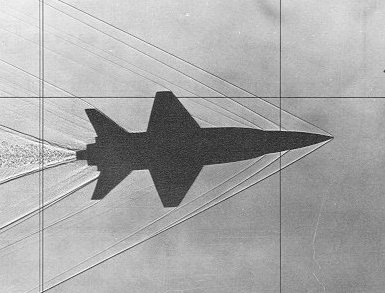
\includegraphics[width=0.8\hsize]{graphics/i-5-1}
\end{center}
\caption{"Uberschallstr"omung um ein "Uberschallflugzeug\label{ueberschall2d}}
\end{figure}

\section{Charakteristiken in h"oheren Dimensionen}
\rhead{Charakteristiken in h"oheren Dimensionen}
Wir wollen jetzt die Frage nach den Charakteristiken in h"oheren Dimensionen
stellen. Um die Diskussion "uberschaubar zu halten, beschr"anken wir uns auf
das dreidimensionale Problem. Die gefundenen Schlussfolgerungen 
lassen sich sofort auf beliebig viele Dimensionen verallgemeinern.

\subsection{Problemstellung}
Das Cauchy-Problem f"ur eine partielle Differentialgleichung der
Form
\[
\sum_{i,j=1}^3a_{ij}\partial_i\partial_ju+\sum_{i=1}^3b_i\partial_iu+cu=f
\]
besteht darin, dass auf einer Fl"ache, die zum Beispiel durch
eine Gleichung
\[
\omega(x_1,x_2,x_3)=0
\]
gegeben werden kann,
die Funktionswerte von $u$ vorgegeben werden, sowie die ersten
Ableitungen in eine Richtung senkrecht auf die Fl"ache.
Diese Ableitung kann mit Hilfe des Gradienten berechnet werden:
\[
\frac{\partial u}{\partial n}=\operatorname{grad}u\cdot \frac{\operatorname{grad}\omega}{|\operatorname{grad}\omega|}
\]
Die L"osung h"angt wieder davon ab, ob die Differentialgleichung
und die Anfangsbedingungen die zweiten Ableitungen von $u$ bereits
eindeutig bestimmen.

\subsection{Ein Spezialfall}
Wir betrachten wieder den Spezialfall, in dem die Anfangswerte auf der
Ebene $x_1=0$ vorgebeben sind, also
\begin{align*}
u(0,x_2,x_3)&=u_0(x_2,x_3),
\\
\partial_1u(0,x_2,x_3)&=h(x_2,x_3)
\end{align*}
Dies entspricht dem Fall $\omega(x_1,x_2,x_3)=x_1$.

Durch die Vorgabe der Anfangswerte in Form der Funktion $u_0$ sind die Ableitungen
$\partial_iu$ f"ur $i=2,3$ ebenfalls festgelegt.
Durch Ableiten der Anfangsbedingungen nach $x_2,\dots,x_3$
sind auch die zweiten Ableitungen 
\[
\partial_i\partial_ju(0,x_2,x_3)\qquad 2\le i\le 3,\;1\le j\le 3
\]
bekannt. Es ist also nur noch $\partial_1^2u$ zu bestimmen.
Die Differentialgleichung kann nach $\partial_1^2u$ aufgel"ost
werden, wenn $a_{11}\ne 0$. Dies ist gleichbedeutend damit, dass
\[
a_{11}=\begin{pmatrix}
1&0&\dots&0
\end{pmatrix}
A
\begin{pmatrix}1\\0\\\vdots\\0\end{pmatrix}
=0.
\]

\subsection{Der allgemeine Fall}
Wir betrachten die Funktion $\omega(x_1,x_2,x_3)$ als die erste
Koordinaten eines neuen Koordinatensystems. Die Koordinaten in diesem
neuen Sytem nennen wir $\omega_1,\dots,\omega_3$, sie sind Funktionen
der alten Koordinaten
\[
\omega_1(x_1,x_2,x_3)=\omega(x_1,x_2,x_3)
,\qquad
\omega_2(x_1,x_2,x_3)
,\qquad
\omega_3(x_1,x_2,x_3)
\]
Die Funktion $u$ kann nat"urlich auch in den neuen Koordinaten geschrieben
werden: $\tilde u(\omega_1,\omega_2,\omega_3)$ hat die Eigenschaft
\[
\tilde u(
\omega_1(x_1,x_2,x_3),
\omega_2(x_1,x_2,x_3),
\omega_3(x_1,x_2,x_3)) = u(x_1,x_2,x_3).
\]
Setzt man dies in die Differentialgleichung ein, ergibt sich
\begin{align*}
\partial_iu
&=
\sum_{k=1}^3
\frac{\partial\tilde u}{\partial \omega_k}
\frac{\partial\omega_k}{\partial x_i}
\\
\partial_i\partial_ju
&=
\sum_{k,l=1}^3
\frac{\partial^2\tilde u}{\partial \omega_k\partial\omega_l}
\frac{\partial\omega_k}{\partial x_i}
\frac{\partial\omega_l}{\partial x_j}
\\
\sum_{i,j=1}^3a_{ij}\partial_i\partial_ju
&=
\sum_{i,j,k,l=1}^3a_{ij}
\frac{\partial^2\tilde u}{\partial \omega_k\partial\omega_l}
\frac{\partial\omega_k}{\partial x_i}
\frac{\partial\omega_l}{\partial x_j}
\\
\sum_{i=1}^3b_i\partial_iu
&=
\sum_{i,k=1}^3b_i
\frac{\partial\tilde u}{\partial \omega_k}
\frac{\partial\omega_k}{\partial x_i},
\end{align*}
die Differentialgleichung f"ur $\tilde u$ in den neuen 
Koordinaten lautet also
\[
\sum_{k,l=1}^3a_{ij}
\biggl(
\sum_{i,j=1}^3a_{ij}
\frac{\partial\omega_k}{\partial x_i}
\frac{\partial\omega_l}{\partial x_j}
\biggr)
\frac{\partial^2\tilde u}{\partial \omega_k\partial\omega_l}
+
\sum_{k=1}^3
\biggl(
\sum_{i=1}^3
b_i
\frac{\partial\omega_k}{\partial x_i}
\biggr)
\frac{\partial\tilde u}{\partial \omega_k}
+c\tilde u
=f.
\]
Die neuen Koeffizienten der zweiten Ableitungen sind also
\[
\tilde a_{kl}=
\sum_{i,j=1}^3a_{ij}
\frac{\partial\omega_k}{\partial x_i}
\frac{\partial\omega_l}{\partial x_j}
\]
Die Fl"ache entspricht in den $\omega$-Koordinaten dem Spezialfall $\omega_1=0$,
die zweiten Ableitungen sind also genau dann eindeutig bestimmt, wenn
der Koeffizient $\tilde a_{11}$ nicht verschwindet. Entlang der durch $\omega$
definierten Fl"ache sind also genau dann die zweiten Ableitungen nicht eindeutig
bestimmt, wenn 
\[
\sum_{i,j=1}^3
a_{ij}
\frac{\partial\omega}{\partial x_i}
\frac{\partial\omega}{\partial x_j}
=
\operatorname{grad}\omega
\cdot
A
\operatorname{grad}\omega
=0
\]
Da der Gradient senkrecht auf der Fl"ache steht, also alle Fl"achen
problematisch, deren Normalen $\vec n$ die Vektorgleichung
\[
\vec n\cdot A\vec n=0
\]
erf"ullen. Diese Vektoren heissen {\em charakteristische Normalen}.

\begin{definition}
Eine durch $\omega(x_1,\dots,x_n)=0$ definierte Fl"ache heisst
charakteristische Fl"ache, wenn auf der Fl"ache
\[
\sum_{i,j=1}^na_{ij}\partial_i\omega\partial_j\omega=0
\]
gilt.
\end{definition}

\subsection{Charakteristische Fl"achen der Wellengleichung}
\begin{figure}
\begin{center}
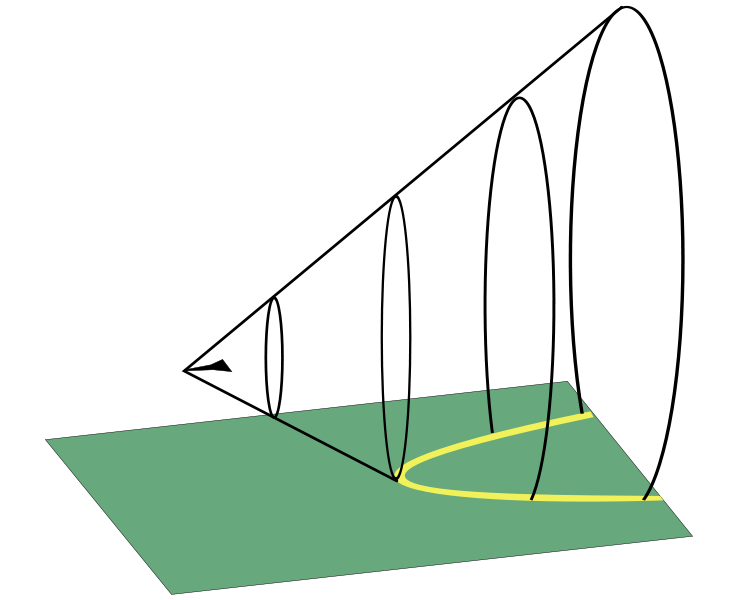
\includegraphics[width=0.8\hsize]{graphics/shock}
\end{center}
\caption{Schockwelle eines "Uberschallfluzeugs als Beispiel einer
charakteristischen Fl"ache von $\partial_t^2u-a^2\Delta u=0$.\label{ueberschallkegel}}
\end{figure}
Wir bestimmen die charakteristischen Fl"achen der
Wellengleichung
\[
\partial_t^2u-a^2\Delta u=0.
\]
Die Koeffizientenmatrix ist
\[
\begin{pmatrix}
1&0&0\\
0&-a^2&0\\
0&0&-a^2
\end{pmatrix},
\]
die charakteristischen Normalen sind also Vektoren $\vec v$, welche die
Gleichung
\[
v_1^2-a^2v_2^2-a^2v_3^2=0
\]
erf"ullen. Diese beschreibt einen Doppelkegel, alle Vektoren, welche mit
der $x_1$-Achse einen festen Winkel einschliessen, sind charakteristische
Normalen. Der Winkel $\alpha$ muss der Bedingung
\[
\cos^2\alpha-a^2\sin^2\alpha=0
\]
gen"ugen, also
\[
\tan\alpha=\pm\frac1a.
\]

Die Winkelbedingung ist die einzige Einschr"ankung an
die charakteristischen Fl"achen,  entsprechend gibt es eine
grosse Vielfalt:
\begin{enumerate}
\item
Jeder Kegel mit halbem "Offnungswinkel $\frac{\pi}2-\alpha$
und Achse parallel zur $x_1$-Achse ist eine charakteristische Fl"ache.
Der Kegel schneidet cie $x_2$-$x_3$-Ebene in einem Kreis, dessen Radius mit
gr"osser werdendem $x_1$ mit der Geschwindigkeit $a$ gr"osser wird.

Abbildung \ref{ueberschallkegel}
zeigt die Schockwelle eines "Uberschallflugzeuges. Schockwellen
als Unstetigkeiten m"ussen sich entlang der charakteristischen Fl"achen ausbreiten,
also entlang eines Kegels.
\item 
Jede Ebene, die mit der $x_1$-Achse einen Winkel von $\frac\pi2-\alpha$
einschliesst, ist charakteristische Fl"ache.
Die Ebene schneidet die $x_2$-$x_3$-Ebene in einer Geraden, die sich
mit der Geschwindigkeit $a$ senkrecht zur Geraden fortbewegt.
Diese charakteristische Fl"ache beschreibt die Fortpflanzung einer
ebenen Welle.
\end{enumerate}


\section{Welche Randwerte beeinflussen die L"osung in einem Punkt?}
\begin{figure}
\centering
\includegraphics{images/kausal-1.pdf}\qquad\qquad%
\includegraphics{images/kausal-2.pdf}
\caption{Randwerte und Punkte des Gebietes, die Einfluss auf einen
Funktionswert der L"osung haben.
Bei einer elliptischen Differentialgleichung $\Delta u=f$
(links)
h"angt jeder Funktionswert von jedem Randwert und von jedem Wert der
Funktion $f$ ab.
Die L"osung einer quasilinearen partiellen Differentialgleichung  (rechts)
im Punkt $x$ h"angt vom Randwert im Anfangspunkt $x_0$ einer Charaketeristik
ab, die durch $x$ verl"auft.
\label{einflussmenge1}}
\end{figure}
\begin{figure}
\centering
\includegraphics{images/kausal-3.pdf}\qquad\qquad%
\includegraphics{images/kausal-4.pdf}
\caption{Randwerte und Punkte des Gebietes, die Einfluss auf einen
Funktionswert der L"osung haben.
Die L"osung einer parabolischen partiellen Differentialgleichung
zur Zeit $t$ h"angt von allen Werten $t'<t$ ab.
Bei einer hyperbolischen partiellen Differentialgleichung beinflussen 
nur die Funktionswerte innerhalb eines vom Punkt $x$ ausgehenden Kegels
von Charakteristiken den Wert der L"osung im Punkt $x$.
\label{einflussmenge2}}
\end{figure}
Mit der entwickelten Theorie ist es jetzt m"oglich, einen Antwort auf die
Frage zu geben, welche Punkte auf dem Rand oder auch im Inneren des Gebietes
einen Einfluss auf die L"osung einer partiellen Differentialgleichung
der Form $Lu=f$ haben.

Im Kapitel~\ref{chapter-elliptisch} haben wir f"ur die L"osung einer
elliptischen partiellen Differentialgleichung eine Formel angegeben,
die $u(x)$ aus allen Randwerten $g$ und der Funktion $f$ in allen 
inneren Punkten berechnet:
\[
u(x)
=
\int_\omega G(x,\xi)f(\xi)\,d\xi
+
\int_{\partial\Omega} \operatorname{grad}_\xi G(x,\xi)g(\xi)\,d\xi.
\]
Eine "Anderung von $g$ in irgend einem Punkt des Randes wird im allgemeinen
Die L"osung $u(x)$ ver"andern, ebenso eine beliebige "Anderung von $f$
(Abbildung~\ref{einflussmenge1}, links).

Im Gegensatz dazu wurde im Kapitel~\ref{chapter-geometrie} gezeigt, 
dass die L"osung einer quasilinearen partiellen Differentialgleichung
erster Ordnung im Punkt $x$ nur vom Wert der Anfangsbedingung im Anfangspunkt
derjenigen Charakteristik abh"angt, die durch $x$ verl"auft
(Abbildung~\ref{einflussmenge1}, rechts).

Die L"osung einer parabolischen partiellen Differentialgleichungen 
kann ebenfalls mit Hilfe einer Greenschen Funktion ausgedr"uckt werden.
Die Formel~(\ref{green-parabolisch}) zeigt, dass die Werte $u(t,x)$
im Allgemeinen von allen Randwerten $g(t',\xi)$ und $f(t',\xi)$
mit $t'<t$ abh"angt (Abbildung~\ref{einflussmenge2}, links).

Die Charakteristischen Fl"achen (Kurven) beantworten die entsprechende
Frage f"ur eine hyperbolische partielle Differentialgleichung.
Die charakteristischen Fl"achen (Kurven), die durch den Punkte $x$ verlaufen,
definieren einen Kegel.
Der Wert $u(x)$ der L"osung im Punkt $x$ h"angt ab von den
Funktionswerten der rechten Seite der Gleichung und den Randwerten
in diesem Kegel
(Abbildung~\ref{einflussmenge2}, rechts).

\section{Zusammenfassung: das Wichtigste in K"urze}
\begin{enumerate}
\item Jede L"osungsfl"ache einer hyperbolischen partiellen Differentialgleichung
kann mit charakteristischen Streifen "uberdeckt werden.
\item Unstetigkeiten breiten sich entlang von Charakteristiken aus.
\item Wie bei quasilinearen partiellen Differentialgleichungen erster
Ordnung kann mit Hilfe der Charakteristiken abgesch"atzt werden, wo
Randwerte und Ableitungen vorgegeben werden m"ussen, damit ein hyperbolisches
Problem gut gestellt ist.
\end{enumerate}

